% 原书第3章 PDF 页29—49，3.2，印刷页201—221。
\section{函数值性状的关联研究}
\subsection{引言}

心电图（ECG）、心音图（phonocardiogram，PCG）、心震图（seismocardiography，SCG）和血氧饱和度等生理性状，为了解人体健康状况提供了重要信息，可用于疾病监测、诊断和管理。例如，心电图是在皮肤表面测得的心肌电活动，反映心跳的频率和规律性。心电图是最常用的心脏检查，具有很高的临床价值。它能提供有关心脏生物学过程及当前状态的宝贵信息，可用于诊断心律失常、心肌梗死及其他心血管疾病。血氧饱和度水平与气流减少程度成正比，会导致睡眠期间睡眠呼吸暂停低通气综合征（Sleep Apnea-Hypopnea Syndrome，SAHS）中呼吸的完全或部分减少。SAHS 是心肌梗死、脑梗死、高血压、心律失常，以及多种心肺系统功能障碍的危险因素。

快速发展的下一代测序（NGS）技术已成为基因表达谱分析的首选平台（Sun and Zhu 2012）。RNA 测序提供了多层次的分辨率及转录组复杂性信息，包括外显子、SNP 和基因组位置层面的表达，以及剪接、异构体表达和等位基因特异性表达。一个基因上的 RNA 测序表达谱，可表示为各基因组位置上的大量读段。这些性状以时间或空间的连续随机函数，或在稠密网格上被观测，称为函数值性状。

函数值性状是高度相关的数据，具有内在的顺序、间隔、平滑变化结构和函数属性。传统方法以汇总值为基础，采用单变量回归和多元回归，原本针对标量性状和常见变异的数量遗传分析而设计，忽略了上述特征。这些方法用汇总统计量度量或表示生理性状。例如，心率（HR）、P--R 间期、QRS 波群时限、QT 间期和 QTc 间期，常被用作心电图遗传分析的性状。生理性状随时间变化，本质上是动态的。它们在多个时间点被重复测量，常以函数或曲线描述。应当比较不同发育阶段对生理性状的遗传控制时间模式。为捕捉生理性状的形态和动态特征，近来发展了联合分析所有动态时间点（性状）的方法，通常称为函数值 QTL 分析（Fusi and Listgarten 2017；Kwak et al. 2015；Hernandez 2015）。

函数值性状关联分析有参数模型和非参数模型两种基本途径。参数模型包括逻辑斯谛生长模型（Ma et al. 2002）和回归模型（Kwak et al. 2014）；非参数模型包括将函数值性状按基函数展开（Yang et al. 2009）、小波展开（Shim and Stephens 2015）、勒让德多项式展开（Das et al. 2011）、函数主成分展开（2015），以及采用径向基函数的高斯过程回归（Fusi and Listgarten 2017）。

过去几年，利用 NGS 数据进行关联研究的新统计方法发展迅速。不过，这些方法未必适用于函数值性状的遗传分析。函数值性状的罕见变异数量遗传分析仍具有挑战。本节介绍响应与预测变量均为函数型的线性模型（functional linear model with functional responses and functional predictors，FLMF），用于基于 NGS 数据的函数值性状数量遗传分析。FLMF 将生理性状随时间变化的取值作为函数型响应，并把一个基因组区域或基因上的基因型谱建模为基因组位置的函数。响应为函数型、预测变量为多元变量的函数型线性模型，可作为 FLMF 的特例，用于常见变异与函数值性状的关联分析。

FLMF 有几个显著特点。第一，它考虑性状的连续变化，保留内在的平滑结构及全部位置层面的遗传信息。第二，它同时利用不同时刻性状之间的相关信息，以及一个基因组区域内全部变异之间的相关信息。第三，它缓解了性状和遗传变异中可能同时存在的多重共线性问题。第四，它将性状函数和基因型函数均按正交特征函数展开，从而大幅降低维数。

\subsection{用于函数值性状关联分析的函数型响应与预测变量线性模型}

为便于讨论，将时间或空间性状统称为函数值性状。为简单起见，考虑第 $i$ 个个体随时间变化的性状 $y_i(t)$，其中 $t\in\mathcal T=[0,T]$，以及基因组区域（或基因）$[a,b]$。设 $s$ 为区域 $S=[a,b]$ 内的一个基因组位置，将第 $i$ 个个体的基因型谱 $x_i(s)$ 定义为
\[
x_i(s)=
\begin{cases}
2P_m(s),&\mathrm{MM},\\
P_m(s)-P_M(s),&\mathrm{Mm},\\
-2P_M(s),&\mathrm{mm},
\end{cases}
\]
其中 $M$ 和 $m$ 是基因组位置 $s$ 处标记的两个等位基因，$P_M(s)$ 和 $P_m(s)$ 分别为等位基因 $M$ 和 $m$ 的频率。响应与预测变量均为函数型的线性模型定义为
\begin{equation}
\begin{aligned}
y_i(t)&=W_i^T\alpha(t)+\int_S x_i(s)\beta(s,t)\,ds+\varepsilon_i(t),\\
&\hspace{1cm}t=t_1,\ldots,t_T,\quad i=1,\ldots,n,
\end{aligned}
\tag{3.44}
\end{equation}
其中 $W_i=[w_{i1},\ldots,w_{id}]^T$ 为协变量向量；$\alpha(t)=[\alpha_1(t),\ldots,\alpha_d(t)]^T$ 为协变量相应的效应向量；$\beta(s,t)$ 是基因组位置 $s$ 和时间 $t$ 处的遗传加性效应函数；$\varepsilon_i(t)$ 是第 $i$ 个个体噪声及未解释效应的残差函数。设 $\eta(t)=[\eta_1(t),\ldots,\eta_k(t)]^T$ 为基函数向量。为将函数型线性模型 (3.44) 转换为标准多元线性模型，考虑性状函数 $y_i(t)$、效应函数 $\alpha(t)$、$\beta(s,t)$ 及基因型函数 $x_i(s)$ 的函数展开。假设表型谱和基因型谱均已中心化。性状函数和基因型函数可按正交归一基函数展开为
\begin{equation}
y_i(t)=\sum_{l=1}^{k_y}y_{il}\eta_l(t)=y_i^T\eta(t),
\tag{3.45}
\end{equation}
以及
\begin{equation}
x_i(s)=\sum_{m=1}^{k_x}x_{im}\theta_m(s),
\tag{3.46}
\end{equation}
其中展开系数 $y_{il}$ 和 $x_{im}$ 由下式估计：
\begin{equation}
y_{il}=\int_0^T y_i(t)\eta_l(t)\,dt
\tag{3.47}
\end{equation}
和
\begin{equation}
x_{im}=\int_S x_i(s)\theta_m(s)\,ds.
\tag{3.48}
\end{equation}
特征函数集合 $\eta_l(t)$ 和 $\theta_m(s)$ 分别由表型函数 $y_i(t)$ 和 $x_i(s)$ 估计。协变量效应函数 $\alpha_j(t)$ 可按特征函数 $\eta_l(t)$ 展开为
\begin{equation}
\alpha_j(t)=\sum_{l=1}^{k_y}\alpha_{jl}\eta_l(t)=\alpha_j^T\eta(t),
\tag{3.49}
\end{equation}
其中 $\alpha_j=[\alpha_{j1},\ldots,\alpha_{jk_y}]^T$。

分别定义协变量效应函数向量和展开系数矩阵为
\[
\alpha(t)=\begin{bmatrix}\alpha_1(t)\\\vdots\\\alpha_d(t)\end{bmatrix},
\qquad
\alpha=\begin{bmatrix}
\alpha_{11}&\cdots&\alpha_{1k_y}\\
\vdots&\vdots&\vdots\\
\alpha_{d1}&\cdots&\alpha_{dk_y}
\end{bmatrix}.
\]
于是有
\begin{equation}
\alpha(t)=\alpha\eta(t).
\tag{3.50}
\end{equation}
类似地，误差函数 $\varepsilon_i(t)$ 也可展开为
\begin{equation}
\varepsilon_i(t)=\sum_{l=1}^{k_y}\varepsilon_{il}\eta_l(t)
=\varepsilon_i^T\eta(t),
\tag{3.51}
\end{equation}
其中 $\varepsilon_i=[\varepsilon_{i1},\ldots,\varepsilon_{ik_y}]^T$。

同理，遗传效应函数 $\beta(s,t)$ 可按两组正交特征函数 $\theta_k(s)$ 和 $\eta_l(t)$ 展开为
\begin{equation}
\beta(s,t)=\sum_{k=1}^{k_x}\sum_{l=1}^{k_y}b_{kl}\theta_k(s)\eta_l(t)
=\theta^T(s)B\eta(t),
\tag{3.52}
\end{equation}
其中 $\theta(s)=[\theta_1(s),\ldots,\theta_{k_\beta}(s)]^T$，$B=(b_{kl})_{k_x\times k_y}$ 为遗传加性效应函数的展开系数矩阵。因此，利用式 (3.46)，积分 $\int_Sx_i(s)\beta(s,t)\,ds$ 可展开为（习题10）
\[
\int_Sx_i(s)\beta(s,t)\,ds
=\int_Sx_i(s)\theta^T(s)\,ds\,B\eta(t)
=x_i^TB\eta(t).
\]
将这些展开代入式 (3.44)，得到
\begin{equation}
y_i^T\eta(T)=W_i^T\alpha\eta(t)+x_i^TB\eta(t)+\varepsilon_i^T\eta(t),
\quad i=1,\ldots,n.
\tag{3.53}
\end{equation}
由于式 (3.53) 应对所有 $t$ 成立，必有
\begin{equation}
y_i^T=W_i^T\alpha+x_i^TB+\varepsilon_i^T,\quad i=1,\ldots,n.
\tag{3.54}
\end{equation}
模型 (3.54) 是一个标准线性模型。这里不用观测数据本身作为响应变量和预测变量的取值，而将它们的展开系数作为线性模型 (3.54) 中响应变量和预测变量的取值。式 (3.54) 还可写为矩阵形式：
\begin{equation}
\begin{aligned}
Y&=W\alpha+XB+\varepsilon,\\
&=A\gamma+\varepsilon,
\end{aligned}
\tag{3.55}
\end{equation}
其中
\[
\begin{gathered}
Y=[y_1,\ldots,y_n]^T,\quad W=[W_1,\ldots,W_n]^T,\quad X=[x_1,\ldots,x_n]^T,\\
\varepsilon=[\varepsilon_1,\ldots,\varepsilon_n]^T,\quad
A=[W,X],\quad \gamma=[\alpha^T,B^T]^T.
\end{gathered}
\]
为估计矩阵 $\gamma$ 中的参数，将真实值 $Y$ 与预测值 $A\hat\gamma$ 之间的误差平方和定义为待最小化的目标函数：
\begin{equation}
F=\Tr\bigl((Y-A\gamma)^T(Y-A\gamma)\bigr)=\Tr(\varepsilon^T\varepsilon).
\tag{3.56}
\end{equation}
利用迹的求导公式，可得
\[
\frac{\partial F}{\partial\gamma}=-A^T(Y-A\gamma).
\]
令 $\partial F/\partial\gamma=0$，得到参数向量 $\gamma$ 的最小二乘估计：
\begin{equation}
\hat\gamma=(A^TA)^{-1}A^TY.
\tag{3.57}
\end{equation}
估计矩阵 $\hat\gamma$ 的最后 $k_x$ 行构成矩阵 $B$ 的估计量。由式 (3.52) 和 (3.57) 得到遗传加性效应函数：
\begin{equation}
\hat\beta(s,t)=\theta^T(s)\hat B\eta(t).
\tag{3.58}
\end{equation}

\subsection{检验统计量}

函数型数量性状关联分析的一个核心问题，是检验基因组区域与函数型数量性状之间的关联。形式上，考虑检验原假设
\begin{equation}
H_0:\beta(s,t)=0,\quad \forall s\in S,\ t\in\mathcal T
\tag{3.59}
\end{equation}
与备择假设
\[
H_a:\beta(s,t)\ne0.
\]
若遗传效应函数 $\beta(s,t)$ 按基函数展开为
\[
\beta(s,t)=\theta^T(s)B\eta(t),
\]
则检验式 (3.59) 中的原假设 $H_0$，等价于检验
\begin{equation}
H_0:B=0.
\tag{3.60}
\end{equation}
为推导检验统计量，首先计算遗传加性效应函数展开系数矩阵估计量的方差。以 $\vecop$ 表示向量化运算。由式 (3.57) 有
\begin{equation}
\begin{aligned}
\vecop(\hat\gamma)
&=\bigl[I_{k_y}\otimes(A^TA)^{-1}A^T\bigr]\vecop(y)\\
&=\vecop(\gamma)+\bigl[I_{k_y}\otimes(A^TA)^{-1}A^T\bigr]\vecop(\varepsilon).
\end{aligned}
\tag{3.61}
\end{equation}
注意
\begin{equation}
\Var\bigl(\vecop(\varepsilon)\bigr)=\Sigma_{k_y}\otimes I_n,
\tag{3.62}
\end{equation}
其中
\begin{equation}
\Sigma_{k_y}=\begin{bmatrix}
\sigma_{11}&\cdots&\sigma_{1k_y}\\
\vdots&\vdots&\vdots\\
\sigma_{k_y1}&\cdots&\sigma_{k_yk_y}
\end{bmatrix}.
\tag{3.63}
\end{equation}
由式 (3.55)，得到
\begin{equation}
\begin{aligned}
y_{ij}&=\sum_{k=1}^{d}W_{ik}\alpha_{kj}+\sum_{k=1}^{k_y}x_{ik}b_{kj}+\varepsilon_{ij},\\
&\hspace{1cm}i=1,\ldots,n,\quad j=1,\ldots,k_y.
\end{aligned}
\tag{3.64}
\end{equation}
方差 $\sigma_{ul}$ 可估计为
\[
\begin{aligned}
\sigma_{ul}={}&\frac{1}{nk_y-dk_y-k_yk_x}\sum_{i=1}^{n}
\left(y_{iu}-\sum_{k=1}^{d}W_{ik}\hat\alpha_{ku}-\sum_{k=1}^{k_y}x_{ik}b_{ku}\right)\\
&\hspace{1cm}\times
\left(y_{il}-\sum_{k=1}^{d}W_{ik}\hat\alpha_{kl}-\sum_{k=1}^{k_y}x_{ik}b_{kl}\right),\\
&\hspace{1cm}u=1,\ldots,k_y,\quad l=1,\ldots,k_y.
\end{aligned}
\]
于是，$\Var(\vecop(\hat\gamma))$ 为
\begin{equation}
\begin{aligned}
\Var\bigl(\vecop(\hat\gamma)\bigr)
&=\bigl[I_n\otimes(A^TA)^{-1}A^T\bigr]\Cov\bigl(\vecop(\varepsilon)\bigr)
   \bigl[I_n\otimes A(A^TA)^{-1}\bigr]\\
&=\bigl[I_n\otimes(A^TA)^{-1}A^T\bigr]\bigl[\Sigma_{k_y}\otimes I_n\bigr]
   \bigl[I_n\otimes A(A^TA)^{-1}\bigr]\\
&=\Sigma_{k_y}\otimes(A^TA)^{-1}.
\end{aligned}
\tag{3.65}
\end{equation}
令
\[
\hat b=\vecop(\hat B),
\]
并令 $\Lambda$ 为取矩阵 $\Var(\vecop(\hat\gamma))$ 最后 $k_yk_x$ 行、最后 $k_yk_x$ 列得到的子矩阵。可定义如下统计量，检验基因组区域与函数型性状的关联：
\begin{equation}
T_F=\hat b^T\Lambda^{-1}\hat b.
\tag{3.66}
\end{equation}
在无关联的原假设下，统计量 $T_F$ 服从中心 $\chi^2_{(k_yk_x)}$ 分布。

\subsection{检验统计量的零分布}

上一节说明，检验统计量 $T_F$ 渐近服从中心 $\chi^2_{(k_yk_\beta)}$ 分布。为考察这一结论的有效性，进行了一系列模拟研究，比较经验水平与名义水平（Lee 2015）。

分别计算仅有罕见等位基因，以及同时有罕见和常见等位基因时的第一类错误率。在计算第一类错误率时，假设由下列模型生成函数型数量性状：
\[
y_i(t_j)=\mu+\varepsilon_i(t_j),
\]
其中 $y_i(t_j)$ 是第 $i$ 个个体在时间 $t_j$ 的性状值；$\mu$ 对所有 $i$ 和 $t_j$ 均为常数；$\varepsilon_i(t_j)$ 是第 $i$ 个个体在时间 $t_j$ 的误差项，由独立标准布朗运动生成。

首先同时考虑常见变异和罕见变异，即变异的整个等位基因频谱。从 NHLBI 外显子组测序项目（Exome Sequencing Project，ESP）中选取五个基因（CDC2L1、GBP3、IQGAP3、TNN、ACTN2），利用2225名个体的变异数据重抽样，生成1,000,000条染色体。这五个基因共包含461个 SNP。从这1,000,000条染色体构成的群体中，抽取1000至2000名个体。计算第一类错误率时，测量性状的时间点数分别为15、20、30和40。共重复5000次模拟。表3.2和表3.3分别汇总了在名义水平 $\alpha=0.05$、$\alpha=0.01$ 和 $\alpha=0.001$ 下，检验罕见变异（MAF $<0.05$）及全部常见和罕见变异关联的统计量在五个基因上的平均第一类错误率。两表表明，总体而言，函数型数量性状分析中检验统计量的第一类错误率与名义 $\alpha$ 水平没有明显差异。

\begin{table}[htbp]
\centering
\origtable{2}{对5个基因取平均，检验仅含罕见变异（MAF $<0.05$）的基因与函数型数量性状关联的统计量的第一类错误率。}
\label{tab:ch03-02}
\begin{tabular}{rrrrr}
\toprule
时间点数 & 样本量 & 0.001 & 0.01 & 0.05\\
\midrule
15 & 1000 & 0.00156 & 0.01232 & 0.05640\\
 & 1250 & 0.00088 & 0.01032 & 0.05320\\
 & 1500 & 0.00120 & 0.01264 & 0.05428\\
 & 1750 & 0.00152 & 0.01296 & 0.05484\\
 & 2000 & 0.00148 & 0.01144 & 0.05492\\
\addlinespace
20 & 1000 & 0.00108 & 0.01164 & 0.05856\\
 & 1250 & 0.00088 & 0.01272 & 0.05876\\
 & 1500 & 0.00088 & 0.01152 & 0.05152\\
 & 1750 & 0.00144 & 0.01056 & 0.05508\\
 & 2000 & 0.00088 & 0.01068 & 0.05220\\
\addlinespace
30 & 1000 & 0.00136 & 0.01200 & 0.05560\\
 & 1250 & 0.00112 & 0.01108 & 0.05232\\
 & 1500 & 0.00092 & 0.01032 & 0.05108\\
 & 1750 & 0.00136 & 0.01032 & 0.05204\\
 & 2000 & 0.00084 & 0.01020 & 0.05116\\
\addlinespace
40 & 1000 & 0.00116 & 0.01184 & 0.05612\\
 & 1250 & 0.00128 & 0.01048 & 0.05344\\
 & 1500 & 0.00124 & 0.01144 & 0.05228\\
 & 1750 & 0.00096 & 0.01032 & 0.04876\\
 & 2000 & 0.00112 & 0.01100 & 0.05092\\
\bottomrule
\end{tabular}
\par\smallskip
\begin{minipage}{0.8\textwidth}\footnotesize
时间点数：测量性状的时间点数量。
\end{minipage}
\end{table}

\begin{table}[htbp]
\centering
\origtable{3}{对5个基因取平均，检验包含全部变异的基因与函数型数量性状关联的统计量的第一类错误率。}
\label{tab:ch03-03}
\begin{tabular}{rrrrr}
\toprule
时间点数 & 样本量 & 0.001 & 0.01 & 0.05\\
\midrule
15 & 1000 & 0.0014 & 0.0130 & 0.0594\\
 & 1500 & 0.0010 & 0.0102 & 0.0552\\
 & 2000 & 0.0006 & 0.0116 & 0.0506\\
\addlinespace
20 & 1000 & 0.0008 & 0.0100 & 0.0532\\
 & 1500 & 0.0014 & 0.0078 & 0.0490\\
 & 2000 & 0.0008 & 0.0090 & 0.0418\\
\addlinespace
30 & 1250 & 0.0012 & 0.0138 & 0.0544\\
 & 1500 & 0.0006 & 0.0092 & 0.0458\\
 & 1750 & 0.0010 & 0.0076 & 0.0426\\
\addlinespace
40 & 1250 & 0.0010 & 0.0126 & 0.0518\\
 & 1500 & 0.0008 & 0.0094 & 0.0482\\
 & 1750 & 0.0008 & 0.0086 & 0.0418\\
\bottomrule
\end{tabular}
\par\smallskip
\begin{minipage}{0.8\textwidth}\footnotesize
时间点数：测量性状的时间点数量。
\end{minipage}
\end{table}

\FloatBarrier

\subsection{统计功效}

为评价响应与预测变量均为函数型的线性模型在检验基因组区域与函数值性状关联方面的表现，利用模拟数据估计其检出真实关联的功效。真实的函数型数量遗传模型如下。考虑位于基因组位置 $s_1,\ldots,s_L$ 的 $L$ 个性状位点。设 $A_s$ 为第 $s$ 个性状位点的风险等位基因，$t_j$ 为测量性状的第 $j$ 个时间点。将下列多重线性回归作为数量性状的加性遗传模型：
\[
y_i(t_j)=\mu+\sum_{s=1}^{L}x_{is}b_s(t_j)+\varepsilon_i(t_j),
\]
其中 $y_i(t_j)$ 是第 $i$ 个个体在时间 $t_j$ 测得的性状值；$\mu$ 为总体均值；$x_{is}$ 是第 $i$ 个个体在第 $s$ 个性状位点的基因型指示变量；$b_s(t_j)$ 是第 $s$ 个性状位点的 SNP 在时间 $t_j$ 的遗传加性效应；误差项 $\varepsilon_i(t_j)$ 由独立标准布朗运动过程生成。将遗传效应 $b_s(t_j)$ 建模为 $b_s(t_j)=b_sb(t_j)$，其中 $b(t_j)=10^{-6}e^t$。对 $b_s$ 考虑隐性和乘性两种遗传模型。假设全部变异位点的相对风险相等，且各变异独立影响性状，即不存在上位性。设 $f_0=1$ 为基线外显率，定义为野生型基因型对性状变异的贡献，并设 $r$ 为风险参数。两种性状模型的遗传加性效应定义为
\[
\begin{aligned}
\text{隐性模型：}\quad &b_s=P_s(r-1)f_0;\\
\text{乘性模型：}\quad &b_s=(rP_s+1-P_s)(r-1)f_0,
\end{aligned}
\]
其中 $P_s$ 是基因组位置 $s$ 处风险等位基因的频率。

为比较功效，还考虑横断面性状模型。其遗传效应定义为遗传效应函数在测量表型的20个时间点上的平均效应：$\bar b_s=b_sb(t_{\mathrm{med}})$，其中 $b(t_{\mathrm{med}})$ 是 $b(t_j)$（$j=1,\ldots,20$）的中位数。横断面模型的性状值由下式生成：
\[
y_i=\mu+\sum_{s=1}^{L}x_{is}\bar b_s+\varepsilon_i.
\]

从 ESP 数据集中选取欧洲裔的2225名个体，利用其基因 TNN 中的变异（88个罕见变异和18个常见变异）重抽样，生成100,000名个体。随机选取10\%的变异作为风险变异。乘性性状模型从群体中抽取1000名个体，隐性性状模型抽取2000名个体。功效计算共重复1000次模拟。比较六种方法：对于时程性状数据，考虑性状与基因型均为函数型的 FLM、多个表型的多元回归，以及多个表型的简单回归；对于横断面数据，考虑性状为标量、基因型为函数型的 FLM、单一表型的多元回归，以及单一表型的简单回归。

本研究比较 FLM、横断面模型、多元回归模型和简单线性回归模型的功效曲线。所有比较均重复1000次模拟，并假设全部变异独立且同等地影响性状，即不存在交互作用。图3.17和图3.18分别给出乘性模型与隐性模型下，检验基因组区域中罕见变异关联的六种统计模型的功效曲线。这六种模型为：用于函数值性状、响应与预测变量均为函数型的线性模型（FLMF）；函数值性状的多重线性模型（MLMF）；函数值性状的简单回归模型（SRGF）；横断面边际遗传模型中响应为标量、预测变量为函数型的线性模型（FLMC）；横断面边际遗传模型的多重线性模型（MLMC）；以及横断面边际遗传模型的简单回归（SRGC）。

\begin{figure}[htbp]
\centering
\begin{tikzpicture}[x=1cm,y=1cm]
\node[anchor=south west,inner sep=0] at (0,0) {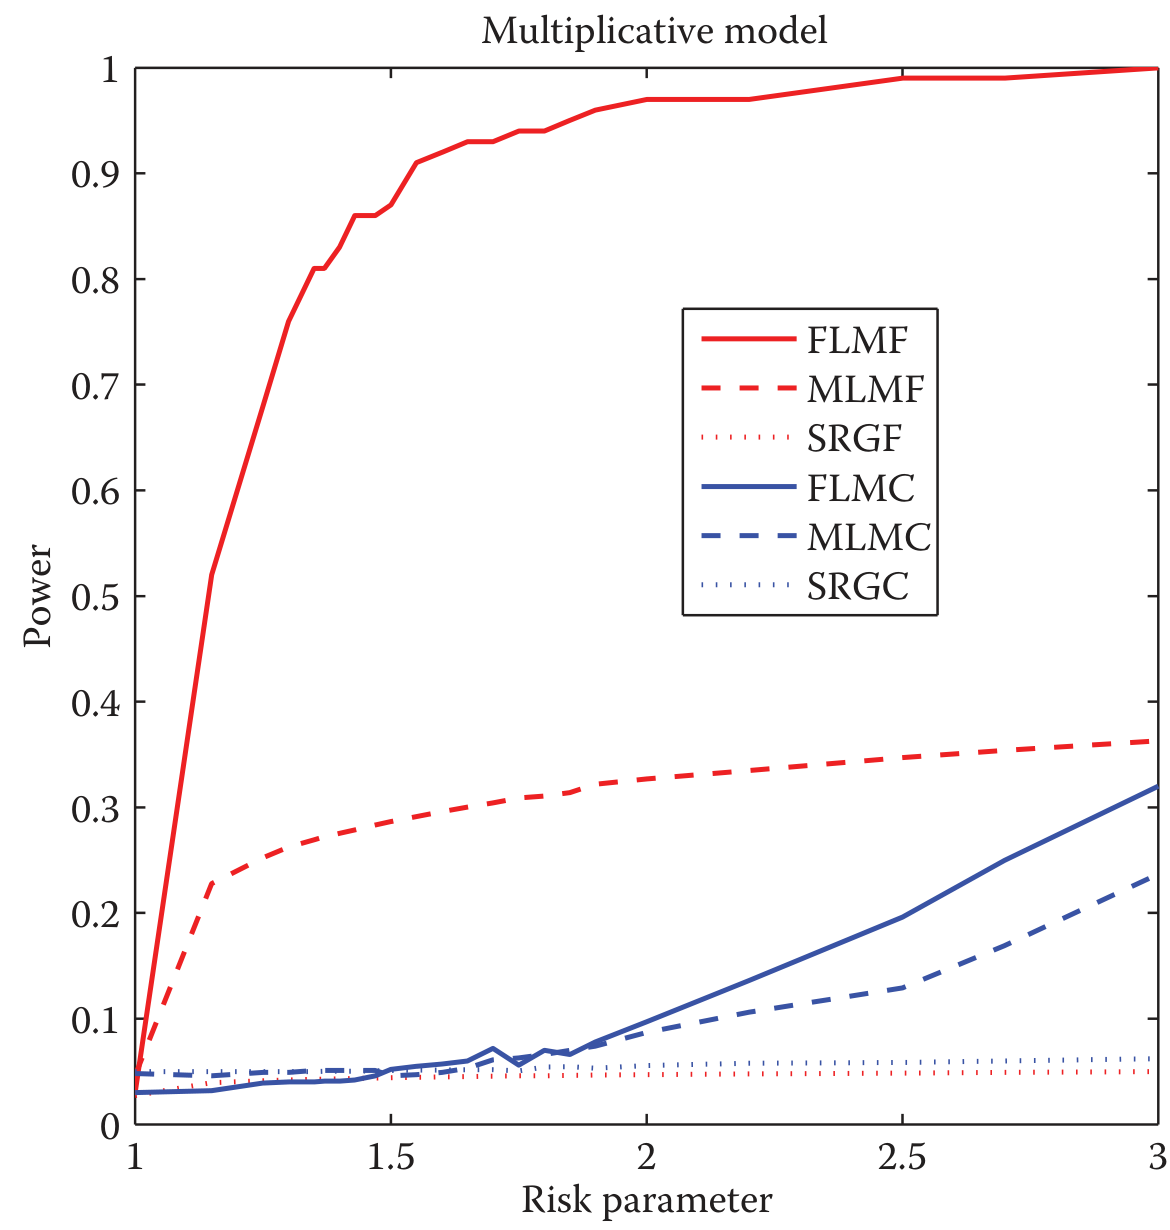
\includegraphics[width=13.0cm]{figures/ch03_fig17_data.png}};
\fill[white] (5.7575,0.0651) rectangle (8.6264,0.5651);
\node[font=\small,rotate=0,inner sep=0] at (7.1919,0.3151) {风险参数};
\fill[white] (0.1867,6.4263) rectangle (0.6978,7.6543);
\node[font=\small,rotate=90,inner sep=0] at (0.4423,7.0403) {统计功效};
\fill[white] (5.3085,13.0487) rectangle (9.2352,13.5487);
\node[font=\small,rotate=0,inner sep=0] at (7.2718,13.2987) {乘性模型};
\end{tikzpicture}
\origfig{17}{乘性模型下，六种模型的统计功效随风险参数的变化曲线。}
\label{fig:ch03-17}
\end{figure}

\begin{figure}[htbp]
\centering
\begin{tikzpicture}[x=1cm,y=1cm]
\node[anchor=south west,inner sep=0] at (0,0) {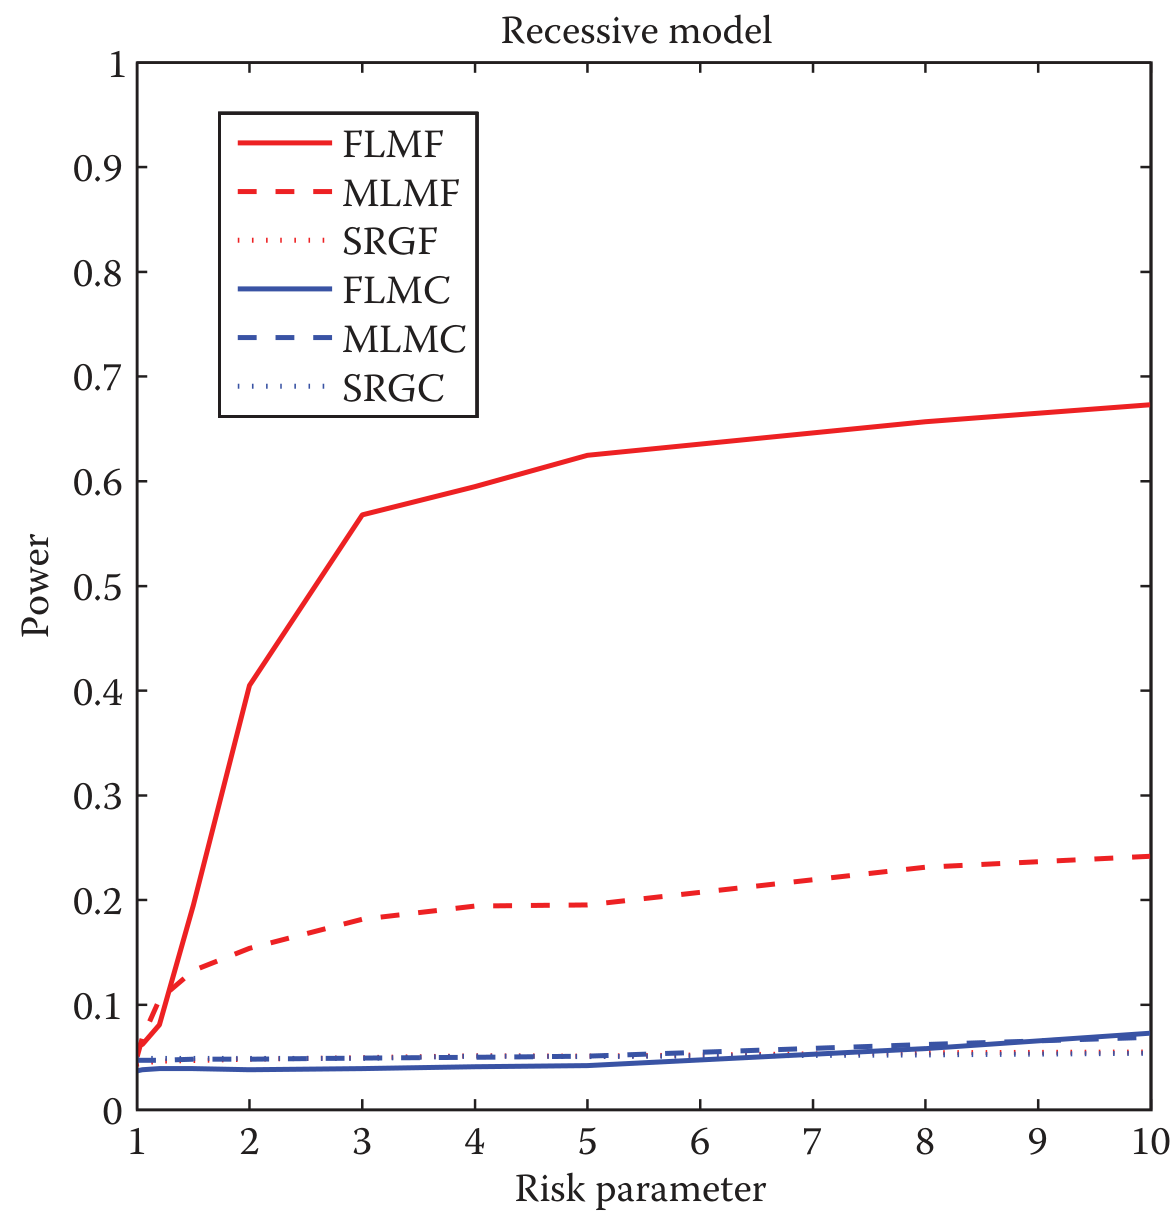
\includegraphics[width=13.0cm]{figures/ch03_fig18_data.png}};
\fill[white] (5.6853,0.0718) rectangle (8.5542,0.5718);
\node[font=\small,rotate=0,inner sep=0] at (7.1197,0.3218) {风险参数};
\fill[white] (0.1615,6.4322) rectangle (0.6726,7.6602);
\node[font=\small,rotate=90,inner sep=0] at (0.4171,7.0462) {统计功效};
\fill[white] (5.5303,12.9375) rectangle (8.6183,13.4375);
\node[font=\small,rotate=0,inner sep=0] at (7.0743,13.1875) {隐性模型};
\end{tikzpicture}
\origfig{18}{隐性模型下，六种模型的统计功效随风险参数的变化曲线。}
\label{fig:ch03-18}
\end{figure}


这些曲线给出显著性水平 $\alpha=0.05$ 下，功效随风险参数的变化。从图中可见几个特点。第一，FLMF 的功效最高。除隐性模型外，即使样本量只有1000，FLMF 仍可检出基因与函数值性状的关联。第二，FLMF 与其余五种模型的功效差异很大。第三，无论是函数值性状，还是横断面边际模型，简单回归（SRGF 和 SRGC）的功效都极低。在大多数情形下，简单回归缺乏检出关联的功效。第四，总体而言，采用函数值方法的检验功效高于传统横断面方法。
\FloatBarrier

\subsection{真实数据分析}

为进一步评价性能，将 FLMF 应用于得克萨斯州斯塔尔县的血氧饱和度研究。血氧饱和度信号按秒测量，一夜共获得35,280次测量。对于阻塞性睡眠呼吸暂停患者，血氧饱和度可为睡眠质量提供重要信息（Lee 2015）。对来自斯塔尔县的833名墨西哥裔美国人，在22,670个基因中共分型406,299个 SNP。由于 FLMF 需要将基因型函数按特征函数展开，每个基因至少需要3个 SNP，因此排除仅含1个或2个 SNP 的基因，最终用于分析的基因总数为17,258。采用 Bonferroni 方法校正多重检验后，判定显著性的 $P$ 值阈值为 $2.90\times10^{-6}$。

为减少纳入分析的测量次数，以每10秒血氧饱和度的均值作为性状值。将基因两侧5 kb 区域内的 SNP 也视为属于该基因。为保证数值稳定性，用奇异值分解计算矩阵的逆，保留能够解释总变异99\%的奇异值数量。为考察 FLMF 的表现，绘制检验的 QQ 图（图3.19）；模型中的 $P$ 值经过性别、年龄和 BMI 调整。

\begin{figure}[htbp]
\centering
\begin{tikzpicture}[x=1cm,y=1cm]
\node[anchor=south west,inner sep=0] at (0,0) {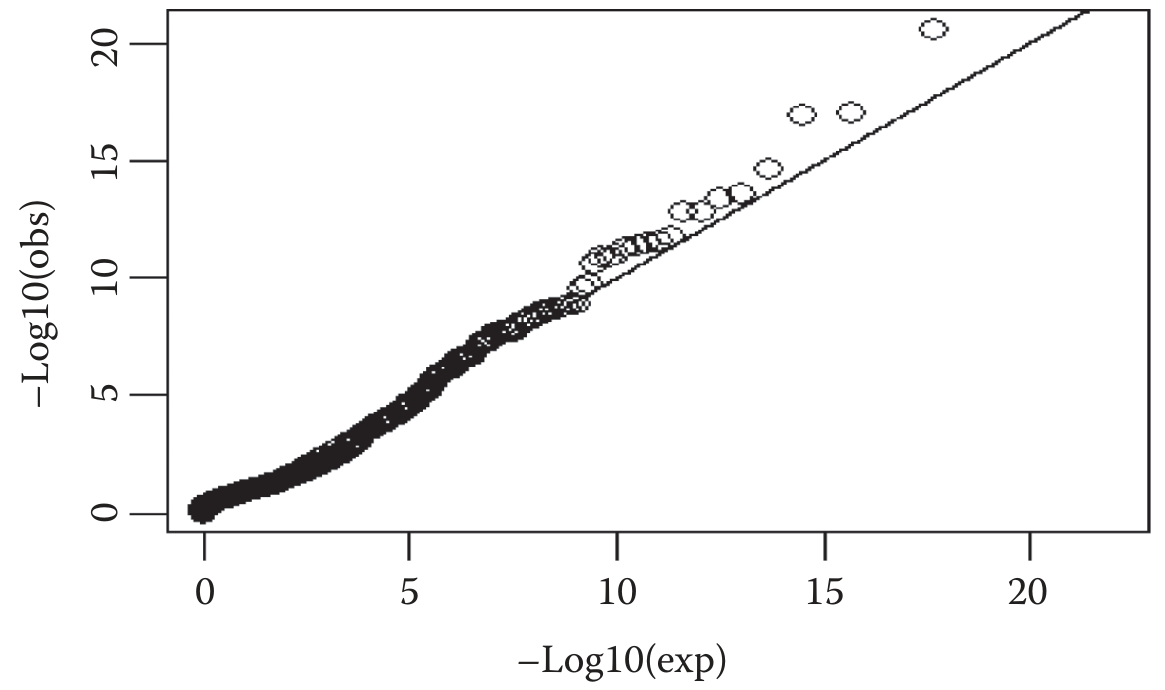
\includegraphics[width=13.0cm]{figures/ch03_fig19_data.png}};
\fill[white] (5.7310,0.0659) rectangle (8.1567,0.5681);
\node[font=\small,rotate=0,inner sep=0] at (6.9439,0.3170) {$-\log_{10}(\text{期望值})$};
\fill[white] (0.1613,3.1085) rectangle (0.6746,5.5141);
\node[font=\small,rotate=90,inner sep=0] at (0.4180,4.3113) {$-\log_{10}(\text{观测值})$};
\end{tikzpicture}
\origfig{19}{QQ 图。}
\label{fig:ch03-19}
\end{figure}


QQ 图表明，FLMF 检测血氧饱和度性状关联时的假阳性率得到控制。共发现65个基因与血氧饱和度函数值性状显著关联，$P$ 值介于 $2.4\times10^{-6}$ 与 $2.5\times10^{-21}$ 之间。为与其他函数值性状关联分析方法比较，表3.4还列出这65个显著基因在全部观测时段的最小 $P$ 值，这些值由各时间点的 MLM 和 SRG 分析计算得到。

本次真实数据分析显示出几个显著特点。第一，FLMF 利用了将表型和基因型均视为函数的优势。它把随时间变化的表型函数分解为时间的正交特征函数，把随位置变化的基因型函数分解为基因组位置的正交特征函数。FLMF 同时降低表型变异和基因型变异的维数，仅需少量特征函数即可表示变异，从而提高检验的统计功效。这个真实数据实例表明，函数值方法（时程数据）可获得比标量值方法（横断面研究）强得多的显著性。第二，为进一步说明函数值统计方法可比传统数量遗传分析具有更高功效，表3.4显示，FLMF 的 $P$ 值小于 MLM 和 SRG 在整夜全部观测时间区间内的最小 $P$ 值。

\begingroup
\small
\setlength{\tabcolsep}{14pt}
\setcounter{table}{3}
\begin{longtable}{lrrr}
\caption{使用 FLMF、MFMF 和 SRGF 计算的65个显著基因的 $P$ 值。}\label{tab:ch03-04}\\
\toprule
\multirow{2}{*}{基因} & \multicolumn{3}{c}{$P$ 值}\\
\cmidrule(lr){2-4}
& FMLF & MLM(min) & SRG(mim)\\
\midrule
\endfirsthead
\multicolumn{4}{c}{表 \thetable\quad（续）}\\
\toprule
基因 & FMLF & MLM(min) & SRG(mim)\\
\midrule
\endhead
\midrule
\multicolumn{4}{r}{（续下页）}\\
\endfoot
\bottomrule
\endlastfoot
MAN1B1 & 2.53E-21 & 1.10E-05 & 6.57E-03\\
TMEM57 & 8.90E-18 & 8.50E-02 & 3.97E-02\\
OR5H15 & 1.28E-17 & 4.21E-03 & 3.29E-02\\
PABPC4L & 2.66E-15 & 1.09E-01 & 7.95E-02\\
ANKLE1 & 2.51E-14 & 6.52E-07 & 2.98E-03\\
TTI2 & 4.64E-14 & 6.82E-02 & 4.57E-03\\
KRTAP4-7 & 1.67E-13 & 1.12E-02 & 5.45E-03\\
WDR90 & 1.73E-13 & 1.49E-10 & 4.56E-04\\
ZER1 & 1.67E-12 & 2.28E-03 & 1.42E-02\\
DPH2 & 3.05E-12 & 3.09E-03 & 2.12E-02\\
B9D2 & 3.43E-12 & 1.07E-01 & 2.87E-02\\
GGT1 & 4.29E-12 & 7.59E-23 & 8.89E-03\\
SGSH & 4.90E-12 & 3.69E-04 & 4.42E-02\\
FAM211B & 1.03E-11 & 1.97E-23 & 8.89E-03\\
FBXO27 & 1.37E-11 & 9.53E-03 & 5.00E-02\\
COA6 & 1.44E-11 & 1.59E-03 & 2.85E-03\\
MAK16 & 2.66E-11 & 3.91E-03 & 9.30E-03\\
CDKN2AIP & 1.69E-10 & 1.62E-01 & 8.54E-02\\
RRM2 & 3.07E-10 & 6.14E-02 & 1.66E-02\\
DTX3L & 1.24E-09 & 2.41E-02 & 4.96E-03\\
C17orf75 & 1.41E-09 & 4.38E-02 & 9.86E-03\\
TAS2R5 & 1.72E-09 & 2.75E-01 & 4.57E-02\\
GIPC1 & 1.93E-09 & 2.29E-02 & 4.41E-02\\
CDC14C & 2.09E-09 & 2.39E-04 & 2.40E-02\\
MIR4520A & 2.49E-09 & 1.06E-03 & 1.44E-01\\
MIR4520B & 2.49E-09 & 1.06E-03 & 1.44E-01\\
PROX2 & 3.63E-09 & 5.24E-03 & 1.15E-02\\
MAFF & 4.04E-09 & 2.17E-03 & 9.18E-04\\
UQCRQ & 5.95E-09 & 1.55E-01 & 2.20E-02\\
LYRM1 & 6.58E-09 & 1.25E-02 & 2.47E-03\\
ZFPM1 & 7.81E-09 & 2.78E-03 & 9.92E-04\\
TMEM50B & 9.59E-09 & 3.14E-23 & 1.27E-03\\
KCNK15 & 1.78E-08 & 1.19E-01 & 7.12E-03\\
EEF1B2 & 1.99E-08 & 4.60E-03 & 1.08E-03\\
SNORA41 & 1.99E-08 & 4.60E-03 & 1.08E-03\\
SNORD51 & 1.99E-08 & 4.60E-03 & 1.08E-03\\
LDLRAP1 & 2.01E-08 & 3.94E-02 & 2.69E-02\\
NEK4 & 2.17E-08 & 3.57E-05 & 5.34E-05\\
COMMD7 & 2.29E-08 & 1.41E-02 & 1.38E-02\\
EEF1A1 & 3.39E-08 & 3.29E-07 & 1.14E-02\\
MIR1-1 & 4.51E-08 & 7.91E-02 & 3.37E-02\\
HMGN4 & 4.63E-08 & 2.05E-03 & 3.47E-03\\
EVPLL & 5.48E-08 & 3.53E-03 & 1.13E-02\\
C22orf26 & 5.60E-08 & 1.17E-02 & 1.52E-03\\
CDC42EP5 & 7.88E-08 & 4.91E-02 & 1.81E-02\\
MIR29C & 1.30E-07 & 2.86E-02 & 8.72E-03\\
LHX2 & 1.95E-07 & 6.47E-03 & 2.77E-04\\
ZNF284 & 2.09E-07 & 1.06E-01 & 7.87E-02\\
RBAKDN & 2.34E-07 & 2.04E-03 & 3.55E-04\\
BAIAP2L2 & 2.44E-07 & 1.91E-02 & 2.14E-03\\
P2RX5 & 2.92E-07 & 6.68E-03 & 1.62E-02\\
P2RX5-TAX & 2.92E-07 & 6.68E-03 & 1.62E-02\\
RELB & 3.01E-07 & 1.10E-02 & 1.29E-02\\
TREML3P & 5.42E-07 & 5.01E-02 & 4.94E-03\\
TSPAN10 & 5.86E-07 & 5.43E-02 & 5.33E-02\\
RPS16 & 6.17E-07 & 2.63E-03 & 6.00E-04\\
GNLY & 8.09E-07 & 1.99E-02 & 1.10E-02\\
LRRC48 & 8.17E-07 & 1.45E-01 & 1.35E-02\\
WSB1 & 9.64E-07 & 7.57E-03 & 6.63E-03\\
GFPT1 & 1.09E-06 & 4.92E-12 & 5.56E-03\\
MIR3677 & 1.13E-06 & 8.67E-02 & 1.40E-02\\
MIR940 & 1.13E-06 & 8.67E-02 & 1.40E-02\\
TOE1 & 1.13E-06 & 6.48E-05 & 6.86E-02\\
TMEM41A & 2.12E-06 & 5.98E-03 & 3.55E-02\\
TPM4 & 2.40E-06 & 1.20E-01 & 8.28E-03\\
\end{longtable}
\endgroup


第三，一个基因中的遗传变异在单个时间点可能仅对血氧饱和度变异有轻微贡献，但仍可能与血氧饱和度曲线显著关联。图3.20即为一例：用 FLMF 检验基因 ANKLE1 与血氧饱和度曲线关联时，$P$ 值为 $2.51\times10^{-14}$；而用 MLM 在各时间点检验时，$P$ 值介于 $6.52\times10^{-7}$ 与 $0.9265$ 之间。共分析3528个时间点，其中188个时间点的 MLM 关联检验 $P$ 值小于 $0.05$。这3528次检验均未显示强关联证据；然而，充分利用表型函数潜在结构的相关性和连续性信息后，确实观测到了基因 ANKLE1 与血氧饱和度曲线的强关联。

\begin{figure}[htbp]
\centering
\begin{tikzpicture}[x=1cm,y=1cm]
\node[anchor=south west,inner sep=0] at (0,0) {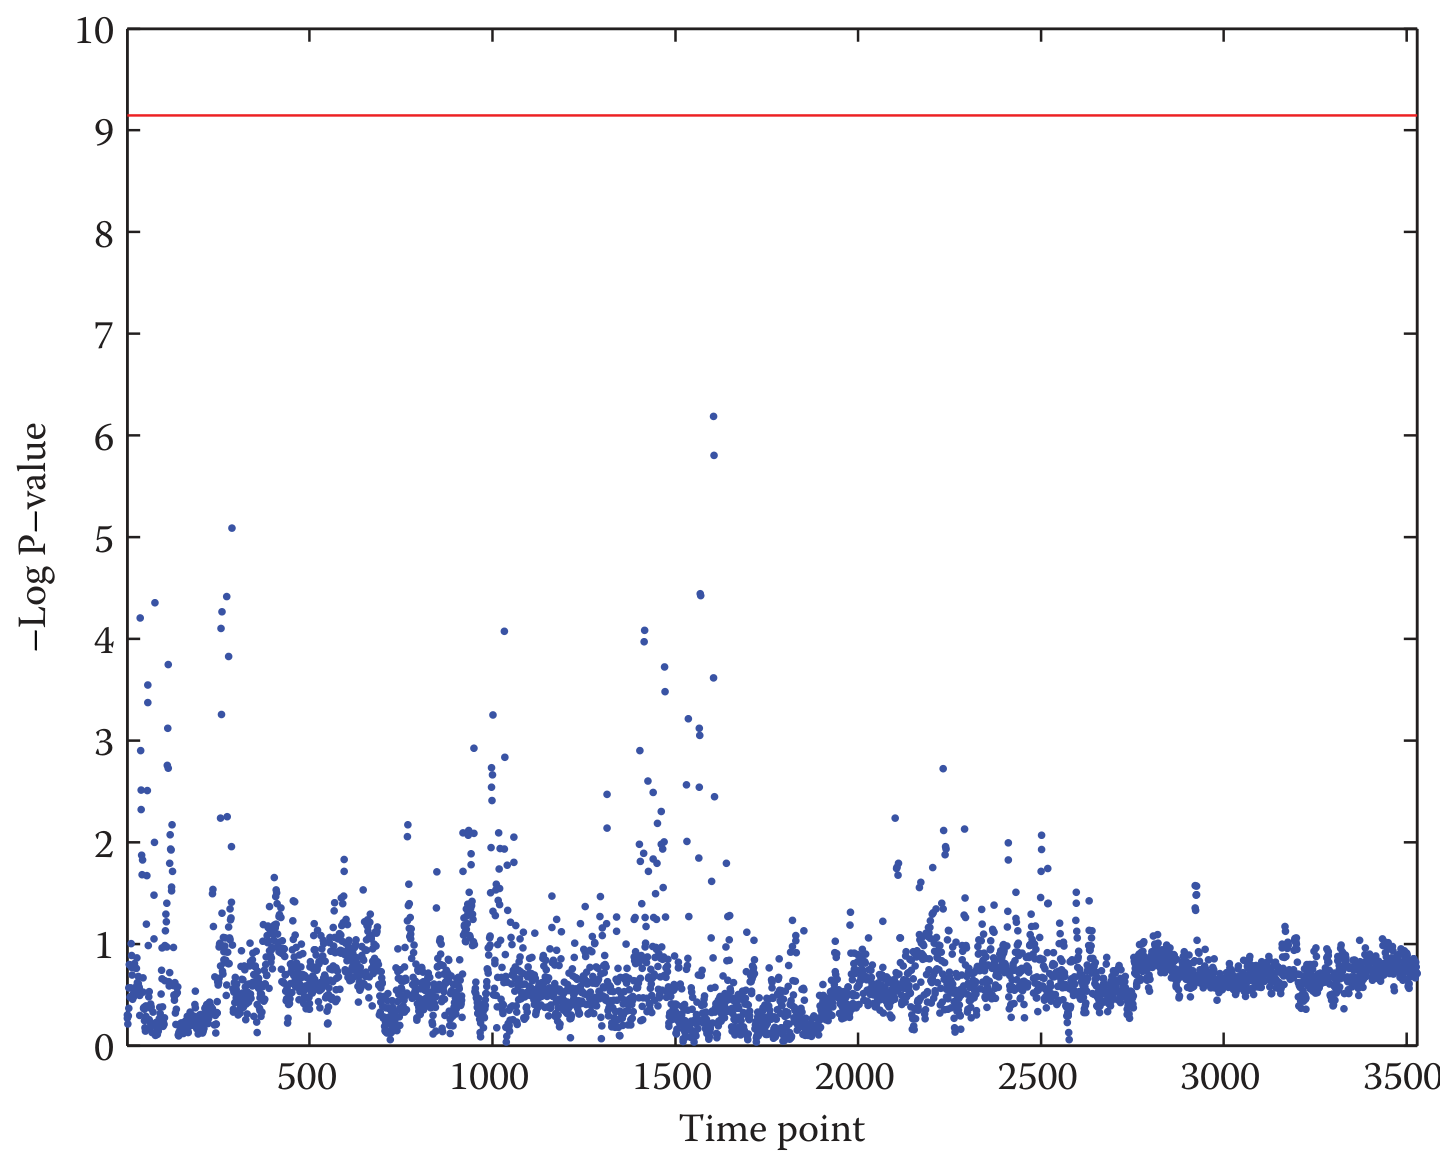
\includegraphics[width=13.8cm]{figures/ch03_fig20_data.png}};
\fill[white] (6.4679,0.0590) rectangle (8.3221,0.4903);
\node[font=\small,rotate=0,inner sep=0] at (7.3950,0.2747) {时间点};
\fill[white] (0.1155,4.8379) rectangle (0.5564,7.0934);
\node[font=\small,rotate=90,inner sep=0] at (0.3360,5.9656) {$-\log P$ 值};
\end{tikzpicture}
\origfig{20}{在各个时间点检验基因 ANKLE1 与血氧饱和度曲线关联所得的 $P$ 值。}
\label{fig:ch03-20}
\end{figure}


第四，传统数量遗传分析计算的是一个固定的检验 $P$ 值，而在函数值性状关联分析中，可以观测随时间变化的 $P$ 值。为说明这一点，图3.21给出整夜每个时间点，使用 MLMT 检验基因 TMEM50B 内全部 SNP 与血氧饱和度关联所得的 $P$ 值随时间 $t$ 的变化。MLM 检验的 $P$ 值随时间快速变化，出现两个显示血氧饱和度显著关联的峰值。在夜间的大部分时间，基因 TMEM50B 中的遗传变异对血氧饱和度的变异并无较大影响。

\begin{figure}[htbp]
\centering
\begin{tikzpicture}[x=1cm,y=1cm]
\node[anchor=south west,inner sep=0] at (0,0) {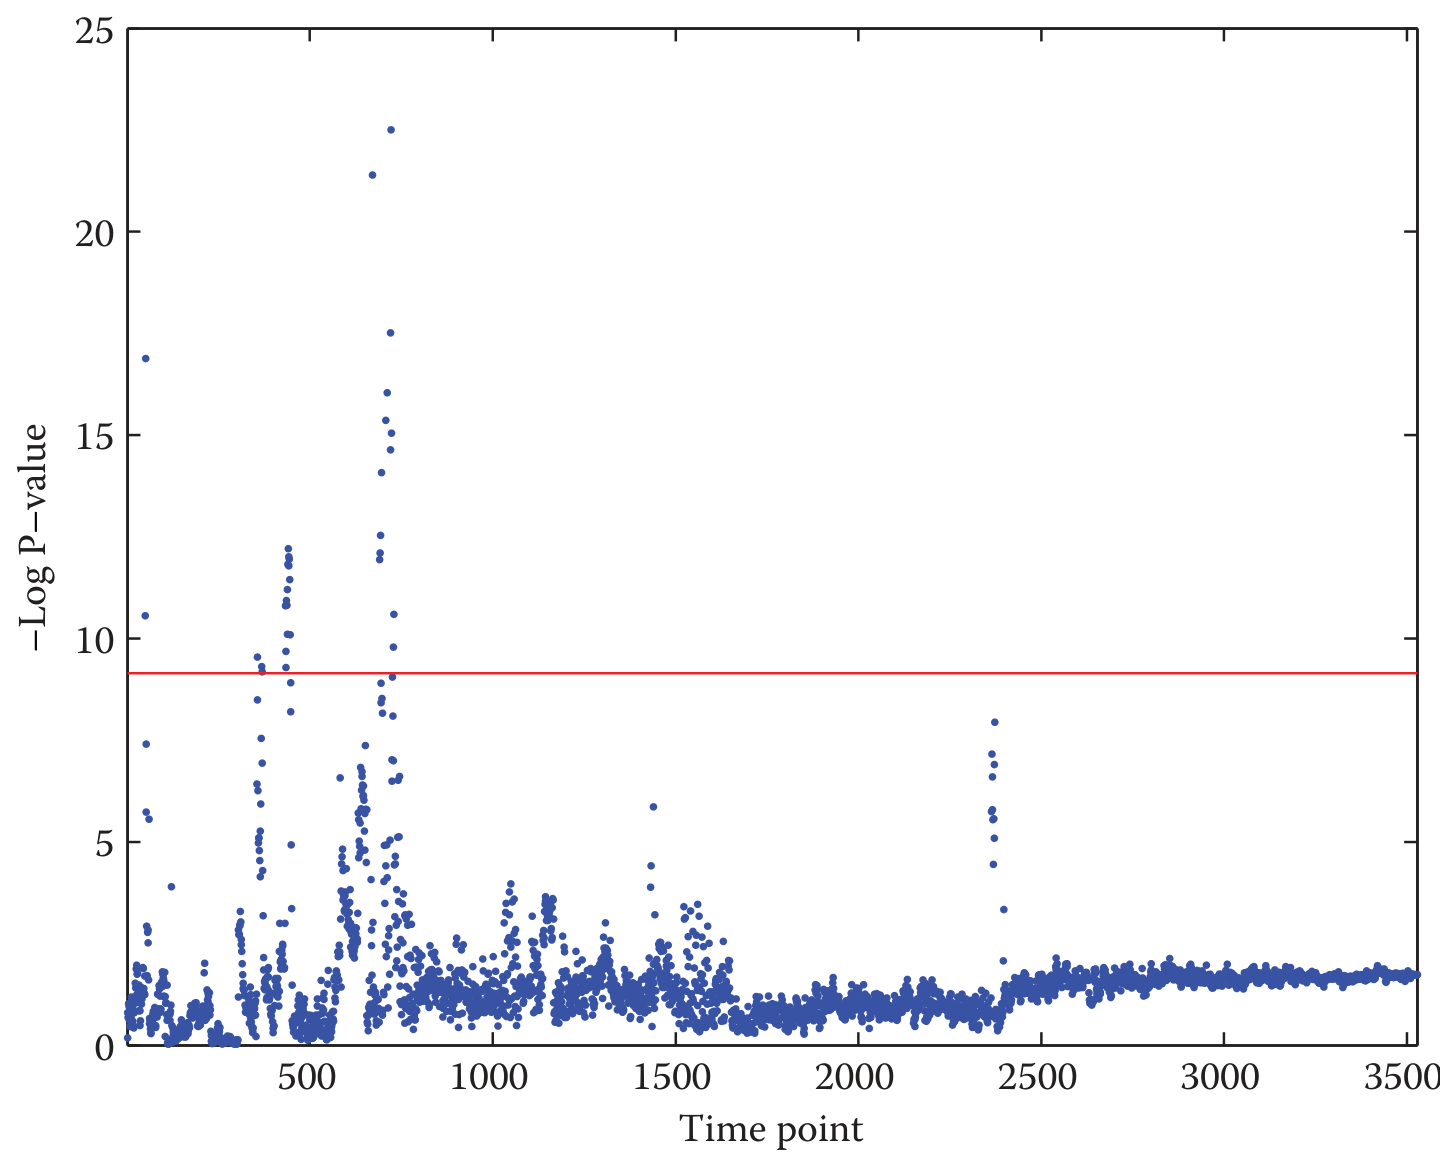
\includegraphics[width=13.8cm]{figures/ch03_fig21_data.png}};
\fill[white] (6.4706,0.0630) rectangle (8.3076,0.4906);
\node[font=\small,rotate=0,inner sep=0] at (7.3891,0.2768) {时间点};
\fill[white] (0.1183,4.8410) rectangle (0.5591,7.0798);
\node[font=\small,rotate=90,inner sep=0] at (0.3387,5.9604) {$-\log P$ 值};
\end{tikzpicture}
\origfig{21}{整夜各时间点，使用 MLMT 检验基因 TMEM50B 内全部 SNP 与血氧饱和度关联所得的 $P$ 值随时间 $t$ 的变化。}
\label{fig:ch03-21}
\end{figure}


FLMF 中的遗传效应具有时空模式，是时间 $t$ 与基因组位置 $s$ 的函数。类似于概率论中的概率密度函数，遗传效应函数可视为单位时间（或指标值）区间和单位基因组区间内的平均遗传效应。相比于基因内部各 SNP 零散的时空遗传效应点，遗传效应函数更易解释。它通常由若干波峰和波谷组成；由于峰值与相邻时间及 SNP 之间存在相关，遗传效应函数峰值处的取值综合了区域内各 SNP 的遗传效应。为说明这一点，图3.22绘出 FLMF 模型中基因 KRTAP4-7（$P<1.67\times10^{-13}$）的遗传效应函数 $\beta(s,t)$ 随时间和基因组位置的变化。遗传效应曲面 $\beta(s,t)$ 完整而详细地提供了时空信息，说明哪些遗传变异以何种方式影响生物学过程的发展，有助于获得新的生物学认识。

\begin{figure}[htbp]
\centering
\begin{tikzpicture}[x=1cm,y=1cm]
\node[anchor=south west,inner sep=0] at (0,0) {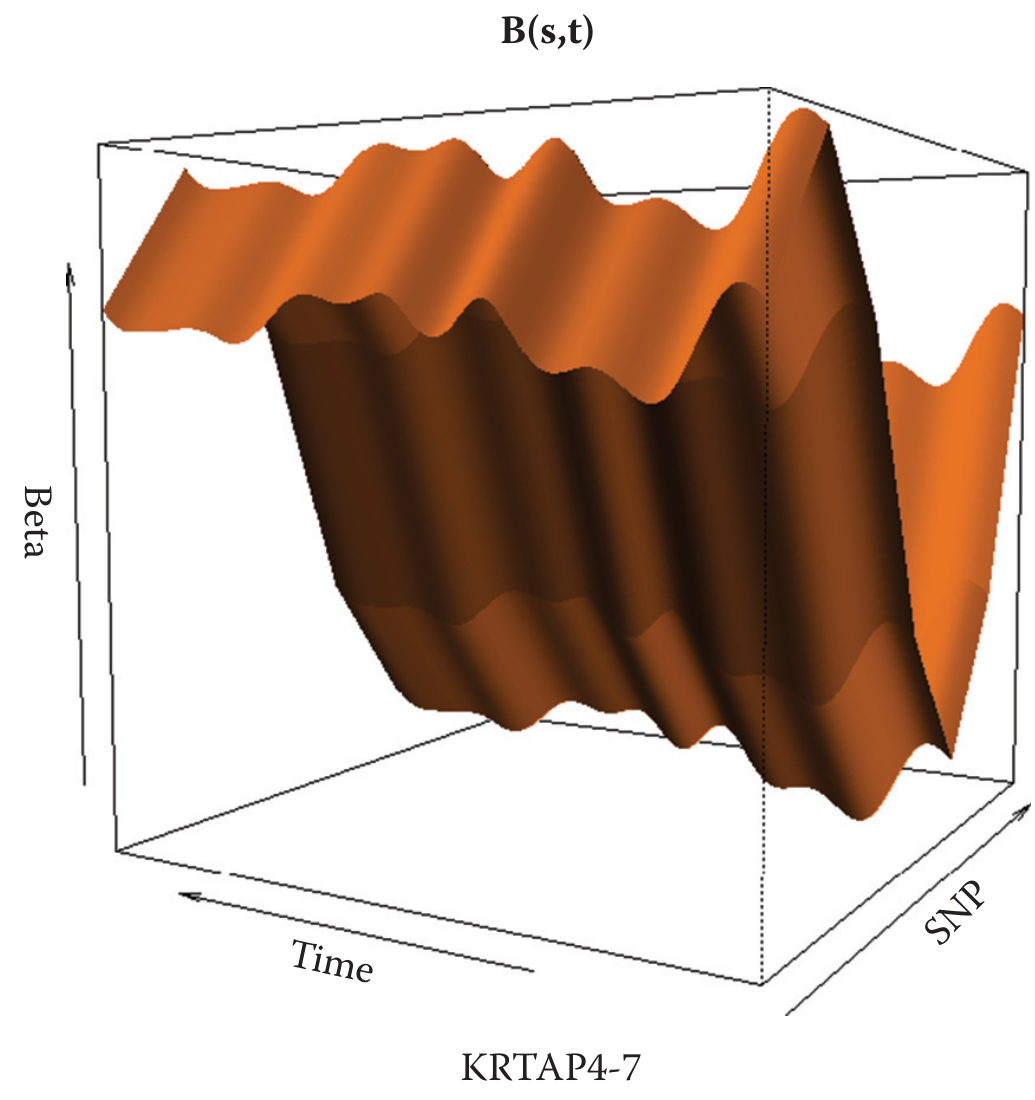
\includegraphics[width=12.0cm]{figures/ch03_fig22_data.png}};
\fill[white] (3.2646,1.2119) rectangle (4.4142,1.9346);
\node[font=\small,rotate=-12,inner sep=0] at (3.8394,1.5732) {时间};
\fill[white] (0.1442,6.2389) rectangle (0.6775,7.1669);
\node[font=\small,rotate=-90,inner sep=0] at (0.4108,6.7029) {$\beta$};
\end{tikzpicture}
\origfig{22}{基因 KPTAP4-7 的遗传效应函数。}
\label{fig:ch03-22}
\end{figure}

\FloatBarrier

\subsection{多个函数值性状的关联分析}

简单函数型线性模型可方便地推广为多重函数型线性模型，用于函数值性状的关联分析。将模型 (3.44) 推广到多个函数值性状，得到
\begin{equation}
\begin{aligned}
y_{ik}(t)&=W_i^T\alpha_k(t)+\int_Sx_i(s)\beta_k(s,t)\,ds+\varepsilon_{ik}(t),\\
&\hspace{.6cm}t=t_1,\ldots,t_T,\quad k=1,\ldots,K,\quad i=1,\ldots,n,
\end{aligned}
\tag{3.67}
\end{equation}
其中 $y_{ik}(t)$ 是第 $i$ 个个体的第 $k$ 个函数值性状；$\alpha_k(t)=[\alpha_{k1}(t),\ldots,\alpha_{kd}(t)]^T$ 为协变量与第 $k$ 个函数值性状相应的效应向量；$\beta_k(s,t)$ 是基因组位置 $s$ 和时间 $t$ 处第 $k$ 个遗传加性效应函数；$\varepsilon_{ik}(t)$ 为第 $i$ 个个体噪声与未解释效应的残差函数。

性状函数和基因型函数按正交归一基函数展开为
\begin{equation}
y_{ik}(t)=\sum_{l=1}^{k_y}y_{ikl}\eta_l(t)=y_{ik}^T\eta(t),
\tag{3.68}
\end{equation}
其中
\[
y_{ikl}=\int_0^Ty_{ik}(t)\eta_l(t)\,dt,\qquad
y_{ik}=[y_{ik1},\ldots,y_{ikk_y}]^T.
\]
协变量效应函数 $\alpha_{kj}(t)$ 可按特征函数 $\eta_l(t)$ 展开为
\begin{equation}
\alpha_{kj}(t)=\sum_{l=1}^{k_y}\alpha_{kjl}\eta_l(t)=\alpha_{kj}^T\eta(t),
\tag{3.69}
\end{equation}
其中 $\alpha_{kj}=[\alpha_{kj1},\ldots,\alpha_{kjk_y}]^T$。定义
\[
\alpha_k=(\alpha_{kjl})_{d\times k_y},\qquad
\alpha=[\alpha_1,\ldots,\alpha_K].
\]
类似地，误差函数 $\varepsilon_{ik}(t)$ 也可展开为
\begin{equation}
\varepsilon_{ik}(t)=\sum_{l=1}^{k_y}\varepsilon_{ikl}\eta_l(t)
=\varepsilon_{ik}^T\eta(t),
\tag{3.70}
\end{equation}
其中 $\varepsilon_{ik}=[\varepsilon_{ik1},\ldots,\varepsilon_{ik_y}]^T$。定义
\begin{equation}
\varepsilon_k=
\begin{bmatrix}\varepsilon_{1k}^T\\\vdots\\\varepsilon_{nk}^T\end{bmatrix}
=\begin{bmatrix}
\varepsilon_{1k1}&\cdots&\varepsilon_{1kk_y}\\
\vdots&\vdots&\vdots\\
\varepsilon_{nk1}&\cdots&\varepsilon_{nkk_y}
\end{bmatrix}.
\tag{3.71}
\end{equation}
遗传效应函数 $\beta_k(s,t)$ 可按两组正交特征函数 $\theta_k(s)$ 和 $\eta_l(t)$ 展开为
\begin{equation}
\beta_k(s,t)=\sum_{j=1}^{k_{xx}}\sum_{l=1}^{k_y}b_{kjl}\theta_j(s)\eta_l(t)
=\theta^T(s)B_k\eta(t),
\tag{3.72}
\end{equation}
其中 $B_k=(b_{kjl})_{k_x\times k_y}$。

因此，式 (3.54) 可推广为
\begin{equation}
y_{ik}^T=W_i^T\alpha_k+x_i^TB_k+\varepsilon_{ik}^T,\quad i=1,\ldots,n.
\tag{3.73}
\end{equation}
模型 (3.73) 可写成矩阵形式：
\begin{equation}
\begin{aligned}
Y&=W\alpha+XB+\varepsilon,\\
&=A\gamma+\varepsilon,
\end{aligned}
\tag{3.74}
\end{equation}
其中
\[
\begin{gathered}
Y=[Y_1\ \cdots\ Y_K],\quad \alpha=[\alpha_1\ \cdots\ \alpha_K],\quad
B=[B_1\ \cdots\ B_K],\\
\varepsilon=[\varepsilon_1\ \cdots\ \varepsilon_K],\qquad
\gamma=\begin{bmatrix}\alpha\\B\end{bmatrix},
\end{gathered}
\]
$W$、$X$ 和 $A$ 的定义同前。注意参数可以分解为
\[
\gamma=[\gamma_1\ \cdots\ \gamma_K]
=\begin{bmatrix}\alpha_1&\cdots&\alpha_K\\B_1&\cdots&B_K\end{bmatrix}.
\]
同样，参数向量 $\gamma$ 的最小二乘估计为（习题3）
\begin{equation}
\hat\gamma=(A^TA)^{-1}A^TY,
\tag{3.75}
\end{equation}
以及
\begin{equation}
\hat\gamma_k=(A^TA)^{-1}A^TY_k,\quad k=1,\ldots,K.
\tag{3.76}
\end{equation}
定义
\[
\vecop(\varepsilon)=\begin{bmatrix}\vecop(\varepsilon_1)\\\vdots\\\vecop(\varepsilon_K)\end{bmatrix},
\qquad
\Sigma=\Var\bigl(\vecop(\varepsilon)\bigr)
=\begin{bmatrix}\Sigma_{11}&\cdots&\Sigma_{1K}\\\vdots&\vdots&\vdots\\\Sigma_{K1}&\cdots&\Sigma_{KK}\end{bmatrix},
\]
其中
\[
\begin{gathered}
\Sigma_{kv}=\Sigma^{kv}\otimes I_n,\qquad
\Sigma^{kv}=\begin{bmatrix}
\sigma_{11}^{(k,v)}&\cdots&\sigma_{1k_y}^{(k,v)}\\
\vdots&\vdots&\vdots\\
\sigma_{k_y1}^{(k,v)}&\cdots&\sigma_{k_yk_y}^{(k,v)}
\end{bmatrix},\\
\Sigma=\Sigma_*\otimes I_n,\qquad
\Sigma_*=\begin{bmatrix}
\Sigma^{11}&\cdots&\Sigma^{1K}\\
\vdots&\vdots&\vdots\\
\Sigma^{K1}&\cdots&\Sigma^{KK}
\end{bmatrix}.
\end{gathered}
\]
模型 (3.74) 也可写为
\begin{equation}
\begin{aligned}
y_{ikj}&=\sum_{l=1}^{d}w_{il}\alpha_{klj}+\sum_{l=1}^{k_y}x_{il}b_{klj}+\varepsilon_{ikj},\\
&\hspace{.6cm}i=1,\ldots,n,\quad k=1,\ldots,K,\quad j=1,\ldots,k_y.
\end{aligned}
\tag{3.77}
\end{equation}
方差 $\sigma_{ul}^{(k,v)}$ 可估计为
\[
\begin{aligned}
\hat\sigma_{ul}^{(k,v)}&=\frac{1}{nk_y-dk_y-k_yk_x}
\sum_{i=1}^{n}\hat\varepsilon_{iku}\hat\varepsilon_{ivl},\\
&\hspace{.6cm}u,l=1,\ldots,k_y,\quad k,v=1,\ldots,K.
\end{aligned}
\]
式 (3.75) 可写为
\begin{equation}
\hat\gamma=\begin{bmatrix}\hat\alpha\\\hat B\end{bmatrix}
=\begin{bmatrix}C_1\\C_2\end{bmatrix}Y,
\tag{3.78}
\end{equation}
其中 $C_1$ 和 $C_2$ 分别由矩阵 $(A^TA)^{-1}A^T$ 的前 $d$ 行和最后 $k_x$ 行构成。因此，式 (3.78) 给出
\begin{equation}
\hat B=C_2Y.
\tag{3.79}
\end{equation}
令
\begin{equation}
\hat b=\vecop(\hat B)=(I\otimes C_2)\vecop(Y).
\tag{3.80}
\end{equation}
注意
\begin{equation}
\Cov\bigl(\vecop(Y)\bigr)=\Cov\bigl(\vecop(\varepsilon)\bigr).
\tag{3.81}
\end{equation}
由式 (3.80) 和 (3.81)，可得
\begin{equation}
\begin{aligned}
\Lambda=\Var\bigl(\vecop(\ddot b)\bigr)
&=[I\otimes C_2]\Cov\bigl(\vecop(Y)\bigr)[I\otimes C_2^T]\\
&=[I\otimes C_2][\Sigma_*\otimes I_n][I\otimes C_2^T]\\
&=\Sigma_*\otimes(C_2\cdot C_2^T).
\end{aligned}
\tag{3.82}
\end{equation}
现考虑检验原假设
\begin{equation}
H_0:\beta_k(s,t)=0,\quad \forall s\in S,\ t\in\mathcal T,\quad k=1,\ldots,K
\tag{3.83}
\end{equation}
与备择假设
\[
H_a:\beta_k(s,t)\ne0,\quad \text{至少对一个 }k\in(1,\ldots,K)\text{ 成立。}
\]
检验式 (3.83) 中的原假设 $H_0$，等价于检验
\begin{equation}
H_0:B_k=0,\quad k=1,\ldots,K.
\tag{3.84}
\end{equation}
可定义如下统计量，检验基因组区域与 $K$ 个函数型性状的关联：
\begin{equation}
T_F=\hat b^T\Lambda^{-1}\hat b.
\tag{3.85}
\end{equation}
在无关联的原假设下，统计量 $T_F$ 服从中心 $\chi^2_{(k_yk_xK)}$ 分布。
\FloatBarrier
